\chapter{Background}
\section{Turing Machine}
\subsection{Introduction to Turing Machines}
A \emph{Turing Machine} (TM) is a collection $(Q, \Sigma, \delta, q_0)$, where:
\begin{itemize}
    \item $Q$ is a set of \emph{states}, including the \emph{accept state} $A$ and \emph{reject state} $R$;
    \item $\Sigma$ is the set of \emph{letters}, which does not include the \texttt{blank} symbol;
    \item $\delta \colon Q \setminus \{A, R\} \times \Sigma^+ \to Q \times \Sigma^+ \times \{\texttt{left}, \texttt{right}\}$, where $\Sigma^+ = \Sigma \cup \{\texttt{blank}\}$, is the \emph{transition function}; and
    \item $q_0 \in Q$ is the \emph{starting state}.
\end{itemize}
Although based on Turing's work on \cite{turing1936computable}, this definition, along with others in this section, have been adapted from \cite{hopcroft2001automata}. This variant of TMs was shown to be equivalent to Turing's definition in \cite{wang1957variant}.

\begin{figure}[htb]
    \centering
    \begin{subfigure}{0.45\textwidth}
        \centering
        \begin{tikzpicture}
            \node[state, accepting] (q0) at (0, 0) {$q_0$};
            \node[state] (q1) at (2.5, 0) {$q_1$};
            \node[state, fill=green, opacity=0.6] (A) at (5, -1) {$A$};
            \node[state, fill=red, opacity=0.6] (R) at (5, 1) {$R$};
    
            \draw[->] (q0) edge[loop above] node[text width=1.5cm, align=center] {$0 \to 0, R$ $1 \to 1, R$} (q0);
            \draw[->] (q0) -- node[above] {$\# \to \#, L$} (q1);
            \draw[->] (q1) -- node[below, rotate=-20] {$0 \to \#, L$} (A);
            \draw[->] (q1) -- node[above, rotate=20, text width=1.5cm, align=center] {$1 \to 1, L$ $\# \to \#, L$} (R);
        \end{tikzpicture}
        \caption{Full notation}
    \end{subfigure}
    \hfill
    \begin{subfigure}{0.45\textwidth}
        \centering
        \begin{tikzpicture}
            \node[state, accepting] (q0) at (0, 0) {$q_0$};
            \node[state] (q1) at (2.5, 0) {$q_1$};
            \node[state, fill=green, opacity=0.6] (A) at (5, -1) {$A$};
            \node[state, fill=red, opacity=0.6] (R) at (5, 1) {$R$};
    
            \draw[->] (q0) edge[loop above] node {$0|1, R$} (q0);
            \draw[->] (q0) -- node[above] {$\#, L$} (q1);
            \draw[->] (q1) -- node[below, rotate=-20] {$0 \to \#, L$} (A);
            \draw[->] (q1) -- node[above, rotate=20] {$1|\#, L$} (R);
        \end{tikzpicture}
        \caption{Shorthand notation}
    \end{subfigure}
    \caption{A FSM representation of a TM that accepts binary numbers divisible by 2.}
    \label{fig:tm_isDiv2}
\end{figure}

We can represent a TM as a \emph{finite state machine} (FSM). This is a directed graph, with vertices as states and edges as transitions. An example is given in Figure \ref{fig:tm_isDiv2}. In this case, the alphabet $\Sigma = \{0, 1\}$. The \texttt{blank} symbol is denoted by $\#$. The initial state is denoted by $q_0$; the accept state $A$ and the reject state $R$. Every edge corresponds to an evaluation of the transition function $\delta$, e.g. $\delta(q_1, 0) = (A, \texttt{blank}, \texttt{left})$. 

The figure presents two ways of representing a FSM- subfigure (a) shows all the transitions, while subfigure (b) only shows the transitions where the tapehead value is getting changed. It also combines letters with similar transitions. We will make use of the shorthand notation.

\subsection{Executing a TM on a tape}
Let $\Sigma$ be an alphabet. A \emph{tape} $T$ on $\Sigma$ is a function $T\colon \mathbb{Z} \to \Sigma^+$. That is, the tape has infinite entries in both directions. Moreover, each tape entry contains a value from the alphabet, or the \texttt{blank} symbol. 

\begin{figure}[htb]
    \centering
    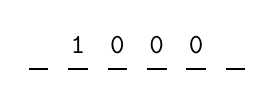
\begin{tikzpicture}
        \foreach \x[count=\i] in {, 1, 0, 0, 0, } {
            \draw[thick] (\i*0.5-0.25, 0) -- (\i*0.5, 0);
            \node at (\i*0.5-0.125, 0.3) {\texttt{\x}};
        }
    \end{tikzpicture}
    \caption{A TM tape on $\{0, 1\}$.}
    \label{fig:tape_example}
\end{figure}
We can represent a tape using a figure. For instance, let $\Sigma = \{0, 1\}$, and let $T$ be the tape on $\Sigma$ given as follows:
\[T(x) = \begin{cases}
    0 & x \in \{0, 2, 3\} \\
    1 & x \in \{1\} \\
    \texttt{blank} & \text{otherwise}.
\end{cases}\]
Then, Figure \ref{fig:tape_example} represents the tape $T$. We will assume that the first non-blank value is at index 0.

We can execute a TM on a tape. Let $M$ be a TM with alphabet $\Sigma$, and let $T$ be a tape on $\Sigma$. We execute $M$ on $T$ inductively, as follows:
\begin{itemize}
    \item At any point during execution, we maintain 3 objects: a tape on $\Sigma$; a (current) state in $M$; and an index in the tape (called the \emph{tapehead index}).  

    \item At the start, the tape is $T$; the tapehead index is $0$; and the current state is the initial state $q_0$. 
    
    \item At some point during the execution, assume that we have the tape $S$, tapehead index $j$, with \emph{tapehead value} $T(j) = t$, and a non-terminating state $q$ (i.e. not $A$ or $R$). Denote $\delta(q, t) = (q', t', \texttt{dir})$. Then, 
    \begin{itemize}
        \item the next state is $q'$;
        \item the next tape is $S'$, where
        \[S'(x) = \begin{cases}
            t' & x = i \\
            S(x) & \text{otherwise};
        \end{cases}\]
        and
        \item the next tapehead index is $j'$, where
        \[j' = \begin{cases}
            j+1 & \texttt{dir} = \texttt{right} \\
            j-1 & \texttt{dir} = \texttt{left}.
        \end{cases}\]
    \end{itemize}
    If the state $q'$ is not a terminating state, then the execution continues with these 3 objects. Otherwise, execution is terminated with terminating state $q'$.
\end{itemize}

\begin{figure}[htb]
    \centering
    \begin{subfigure}{0.4\textwidth}
        \centering
        \begin{tikzpicture}
            \foreach \x[count=\i] in {, 1, 0, 0, 0, } {
                \draw[thick] (\i*0.5-0.25, 0) -- (\i*0.5, 0);
                \node at (\i*0.5-0.125, 0.3) {\texttt{\x}};
            }
            \draw[->] (2.875, -0.5) -- (2.875, -0.1);
        \end{tikzpicture}
        \caption{}
    \end{subfigure}
    \begin{subfigure}{0.4\textwidth}
        \centering
        \begin{tikzpicture}
            \foreach \x[count=\i] in {, 1, 0, 0, , } {
                \draw[thick] (\i*0.5-0.25, 0) -- (\i*0.5, 0);
                \node at (\i*0.5-0.125, 0.3) {\texttt{\x}};
            }
            \draw[->] (1.875, -0.5) -- (1.875, -0.1);
        \end{tikzpicture}
        \caption{}
    \end{subfigure}
    \caption{Some of the tape states during execution.}
    \label{fig:tm_tape_execution}
\end{figure}
We illustrate this process with the TM in Figure \ref{fig:tm_isDiv2} with the tape in Figure \ref{fig:tape_example}:
\begin{itemize}
    \item Initially, the tape is the given tape; $q_0$ is the current state; and the tapehead index is $0$, with value $1$.
    
    \item According to the FSM, we have $\delta(q_0, 1) = (q_0, 1, R)$. Hence,
    \begin{itemize}
        \item the tape remains unchanged;
        \item $q_0$ is still the current state; and
        \item and the tapehead index becomes $1$, with value \texttt{0}.
    \end{itemize}
    
    \item The transition for \texttt{0} and \texttt{1} are the same with respect to $q_0$. This means that we keep moving to the right, until we end up at a blank symbol. At that point, the state of the tape is given in Figure \ref{fig:tm_tape_execution} (a). The arrow points at the tapehead entry. We are still at the state $q_0$, and the tape has not been altered.
    
    \item Now, since the tapehead value is \texttt{blank}, we move to the left and the current state becomes $q_1$. The tape has still not been changed. The current value is now $0$.
    
    \item We have $\delta(q_1, 0) = (A, \texttt{blank}, L)$. So, 
    \begin{itemize}
        \item the tapehead value changes to from $0$ to blank;
        \item the current state becomes $A$; and
        \item the tapehead pointer move to the left, to index $2$.
    \end{itemize}
    Since $A$ is a terminating state, execution terminates, with result \texttt{accept}. The final tape state is given in Figure \ref{fig:tm_tape_execution} (b).
    
\end{itemize}
So, the TM in Figure \ref{fig:tm_isDiv2} executes as follows:
\begin{itemize}
    \item we use the state $q_0$ to traverse to the first blank symbol (i.e. the end of the string), and then move to the state $q_1$;
    \item at state $q_1$, we accept the string if and only if the current tapehead value is \texttt{0}
\end{itemize}
Hence, this TM accepts binary numbers if and only if they are divisible by 2.

\subsection{TM as a model of computation}
Turing initially proposed TMs as the `correct' model of computation in \cite{turing1936computable}. This result is referred to as the \emph{Church-Turing Thesis}. It is a thesis since it is informal in nature; it is just a \textit{belief} that the correct model of computation is the model given by TMs. 

In this paper, Turing also showed that TMs and $\lambda$-calculus are equivalent. Hence, it follows that $\lambda$-calculus is also the correct model of computation. There have been many other models of computations proposed, such as general recursive functions. It is widely regarded that TMs (and all the equivalent models) represent the correct model of computation. This is because many of the originally proposed models of computation turned out to be equivalent (\cite{copeland2004essential}).

\section{Parser}
A \emph{compiler} is a program that takes source code in a programming language (PL) and translates it into a program in another, target, PL. During the process, the compiler also detects any errors, such as syntax and type errors. 

\begin{figure}[htb]
    \centering
    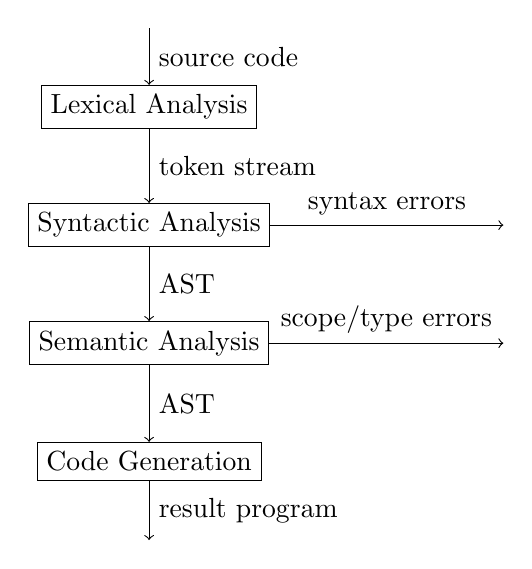
\begin{tikzpicture}
        \node[draw] (LA) at (0, 0) {Lexical Analysis};
        \node[draw] (SA) at (0, -1.5) {Syntactic Analysis};
        \node[draw] (CA) at (0, -3) {Semantic Analysis};
        \node[draw] (CG) at (0, -4.5) {Code Generation};
        
        \draw[->] (0, 1) -- node[right] {source code} (LA);
        \draw[->] (LA) -- node[right] {token stream} (SA);
        
        \draw[->] (SA) -- node[above] {syntax errors} (4.5, -1.5);
        \draw[->] (SA) -- node[right] {AST} (CA);
        \draw[->] (CA) -- node[above] {scope/type errors} (4.5, -3);
        
        \draw[->] (CA) -- node[right] {AST} (CG);
        \draw[->] (CG) -- node[right] {result program} (0, -5.5);
    \end{tikzpicture}
    \caption{The data flow between the compilation phases.}
    \label{fig:compilation_process}
\end{figure}

We will now consider the different phases of the compilation process. This is summarised in Figure \ref{fig:compilation_process}. This figure, along with most of the content in this section, has been adapted from \cite{aho2007compilers}.

\subsection{Lexical Analysis}    
During the compilation process, we first perform \emph{lexical analysis}. In this stage, the source code is enriched to make it ready for parsing. In particular, we generate a stream of source code, which reads the program word by word. Then, it produces a stream of \emph{tokens}. A token is a word in source code along with a label. For instance, consider the mathematical expression \texttt{1 + 2}. We can convert this expression into 3 tokens: \texttt{(1, NUM)}, \texttt{(+, PLUS)} and \texttt{(2, NUM)}. 

\subsection{Syntactic Analysis}

Next, we try to parse the token stream into an \emph{abstract syntax tree} (AST). If there are syntax errors present in the program, then it is not possible to construct an AST. This will be detected during the process, at which point we can throw a syntax error.

\begin{figure}[htb]
    \centering
    \begin{tikzpicture}[
        level 1/.style={sibling distance=4cm},
        level 2/.style={sibling distance=2cm},
    ]
        \node[ellipse, draw] {TIMES}
        child {
            node[ellipse, draw] {PLUS}
            child {
                node[draw] {\texttt{1}}
            }
            child {
                node[draw] {\texttt{2}}
            }
        }
        child {
            node[ellipse, draw] {PLUS}
            child {
                node[draw] {\texttt{3}}
            }
            child {
                node[draw] {\texttt{4}}
            }
        };
    \end{tikzpicture}
    \caption{The AST for the expression \texttt{(1 + 2) * (3 + 4)}}
    \label{fig:AST_example}
\end{figure}

An AST represents the program as a tree. Typically, the internal nodes represent operations, whereas the leaves represent their arguments. The AST for the expression \texttt{(1 + 2) * (3 + 4)} is given in Figure \ref{fig:AST_example}.

There are many ways to parse the stream of tokens. A common method is \emph{recursive-descent parsing}. Here, we have a parser function for each construct in the language, such as a \textit{program}, an \textit{if} command, an \textit{expression}, etc. We look at the next token value and choose the right function.

One way of performing recursive-descent parsing is by \emph{top-down parsing}. In this case, we produce the parent node of the AST and then generate its children. 

The simplest form of recursive-descent parsing is called \emph{predictive parsing}. This applies when the next token determines what structure it is to be parsed. For instance, if we see the token \texttt{if}, then we know we are parsing an \textit{if} command.

\subsection{Semantic Analysis}
Now, we traverse the AST and check that there are no errors in the source code. Typically, there are 2 types of things to check in this stage- \emph{type errors} and \emph{scope errors}. 

In type errors, we check whether the AST has some type mismatch, e.g. \texttt{1 + true}. We can detect this by keeping track of the types of the identifiers and see if they are legal.

In scope errors, we ensure that all the identifiers present in code are defined. To do so, we need to keep track of all the variables that are in scope. In terms of functions, there is a design choice here- we can have all functions in scope from the start, or add them to scope as they are encountered. Another thing to consider is recursion- to allow recursion, the function must be in scope as soon as it is declared.

\subsection{Code Generation}
Finally, we convert the AST into code in the target language. In particular, we traverse the tree and convert each phrase from the source language to the target.
